\documentclass[a4paper,10pt]{article}
\usepackage{fancyhdr}
\usepackage{graphicx}
\usepackage[utf8]{inputenc}
\usepackage{a4wide}
\usepackage{fancyvrb}
%\usepackage{flafter}
\usepackage{multicol} 
     
% Title Page
\title{Technical notes Document}
\author{Jonathan Alvarsson}

\begin{document}
        
    %turns on the fancy heading
    \pagestyle{fancy}	

    %makes the text up in the right corner
    \renewcommand{\sectionmark}[1]{\markboth{#1}{}}

    %emptys header and footer from default values
    \fancyhead{}

    %places the text up in the right corner
    \fancyhead[RO]{\large\textbf{{\leftmark}}}

    %places the page number
    \fancyhead[LO]{\large\textbf{\today}}

    %sets the height of the header
    \headheight=18pt
        
    \setcounter{tocdepth}{3}
        
    \maketitle 
    \newpage 
    
    \tableofcontents 
    \newpage
        
	\section{Persistent classes}
	
    \begin{multicols}{2}
        \noindent The persistent classes, the classes that can be written and
        loaded from the database can be found in the
        \texttt{net.bioclipse.lis.pojos} package (pojo stands for plain old
        java object which is more or less how they are implemented). These
        classes contains a couple of values, getters and setters for these
        values and implementations of \texttt{hashcode()}, \texttt{equals()},
        and \texttt{deepCopy()} and that's about what they contain.
    	
        The persisten classes all extend \texttt{AbstractBaseObject} and in
        some cases also \texttt{AbstractAuditableObject}.
   
        \subsection{Deleting} The persistent classes can't really be deleted.
        They can be marked as deleted and thus later be restored. So when one
        of them is said to be deleted that means that it is marked as deleted.
        There is a somewhat special behavior related to their
        \texttt{delete()}-methods see table \ref{deleting}. 
   
    \end{multicols}

    \begin{table}[hbt]
        
        \begin{center}
        \begin{tabular}{|l|l|}
                \hline
                \textbf{Persistent class} & \textbf{Behavior} \\
                \hline
                \hline
                CellOrigin & Can only be deleted when no 
                             CellSample references it \\
                
                DrugOrigin & Can only be deleted when no 
                             DrugSample references it \\
                             
                Annotation & Also deletes all related 
                             AbstractAnnotationInstances \\
                             
                Experiment & Also deletes all related Plates \\
                
                Instrument & Can only be deleted when no 
                             Measurement references it \\
                             
                InstrumentType & Can only be deleted when no Instrument 
                                 references it \\
                                 
                LayoutWell & Also deletes all related LayoutMarkers \\
                
                MasterPlate & Alse deletes all related Wells, 
                              PlateFunctions and AnnotationInstances \\ 
                              
                Measurement & Also deletes all related Results \\
                
                PlateLayout & Also deletes all related LayoutWells, 
                              PlateFunctions and \\
                            & AnnotationInstances  \\
                            
                Plate       & Also deletes all related Wells, PlateFunctions,
                              and  AnnotationInstances \\
                              
                Project     & Also deletes all related Experiments \\
                
                SampleContainer & Also deletes all related samples and the
                                  related  Worklist \\
                                  
                Well        & Also deletes related SampleMarkers, 
                              WellFunctions and the related\\
                            & SampleContainer \\
                            
                WorkList    & Also deletes all related Operations. \\
                \hline
        \end{tabular}
        \end{center}
        \label{deleting}
        \caption{The behavior of some special persistent classes regarding
                 delete}
    \end{table}
	
    \begin{figure}[hp]
        \begin{center}
            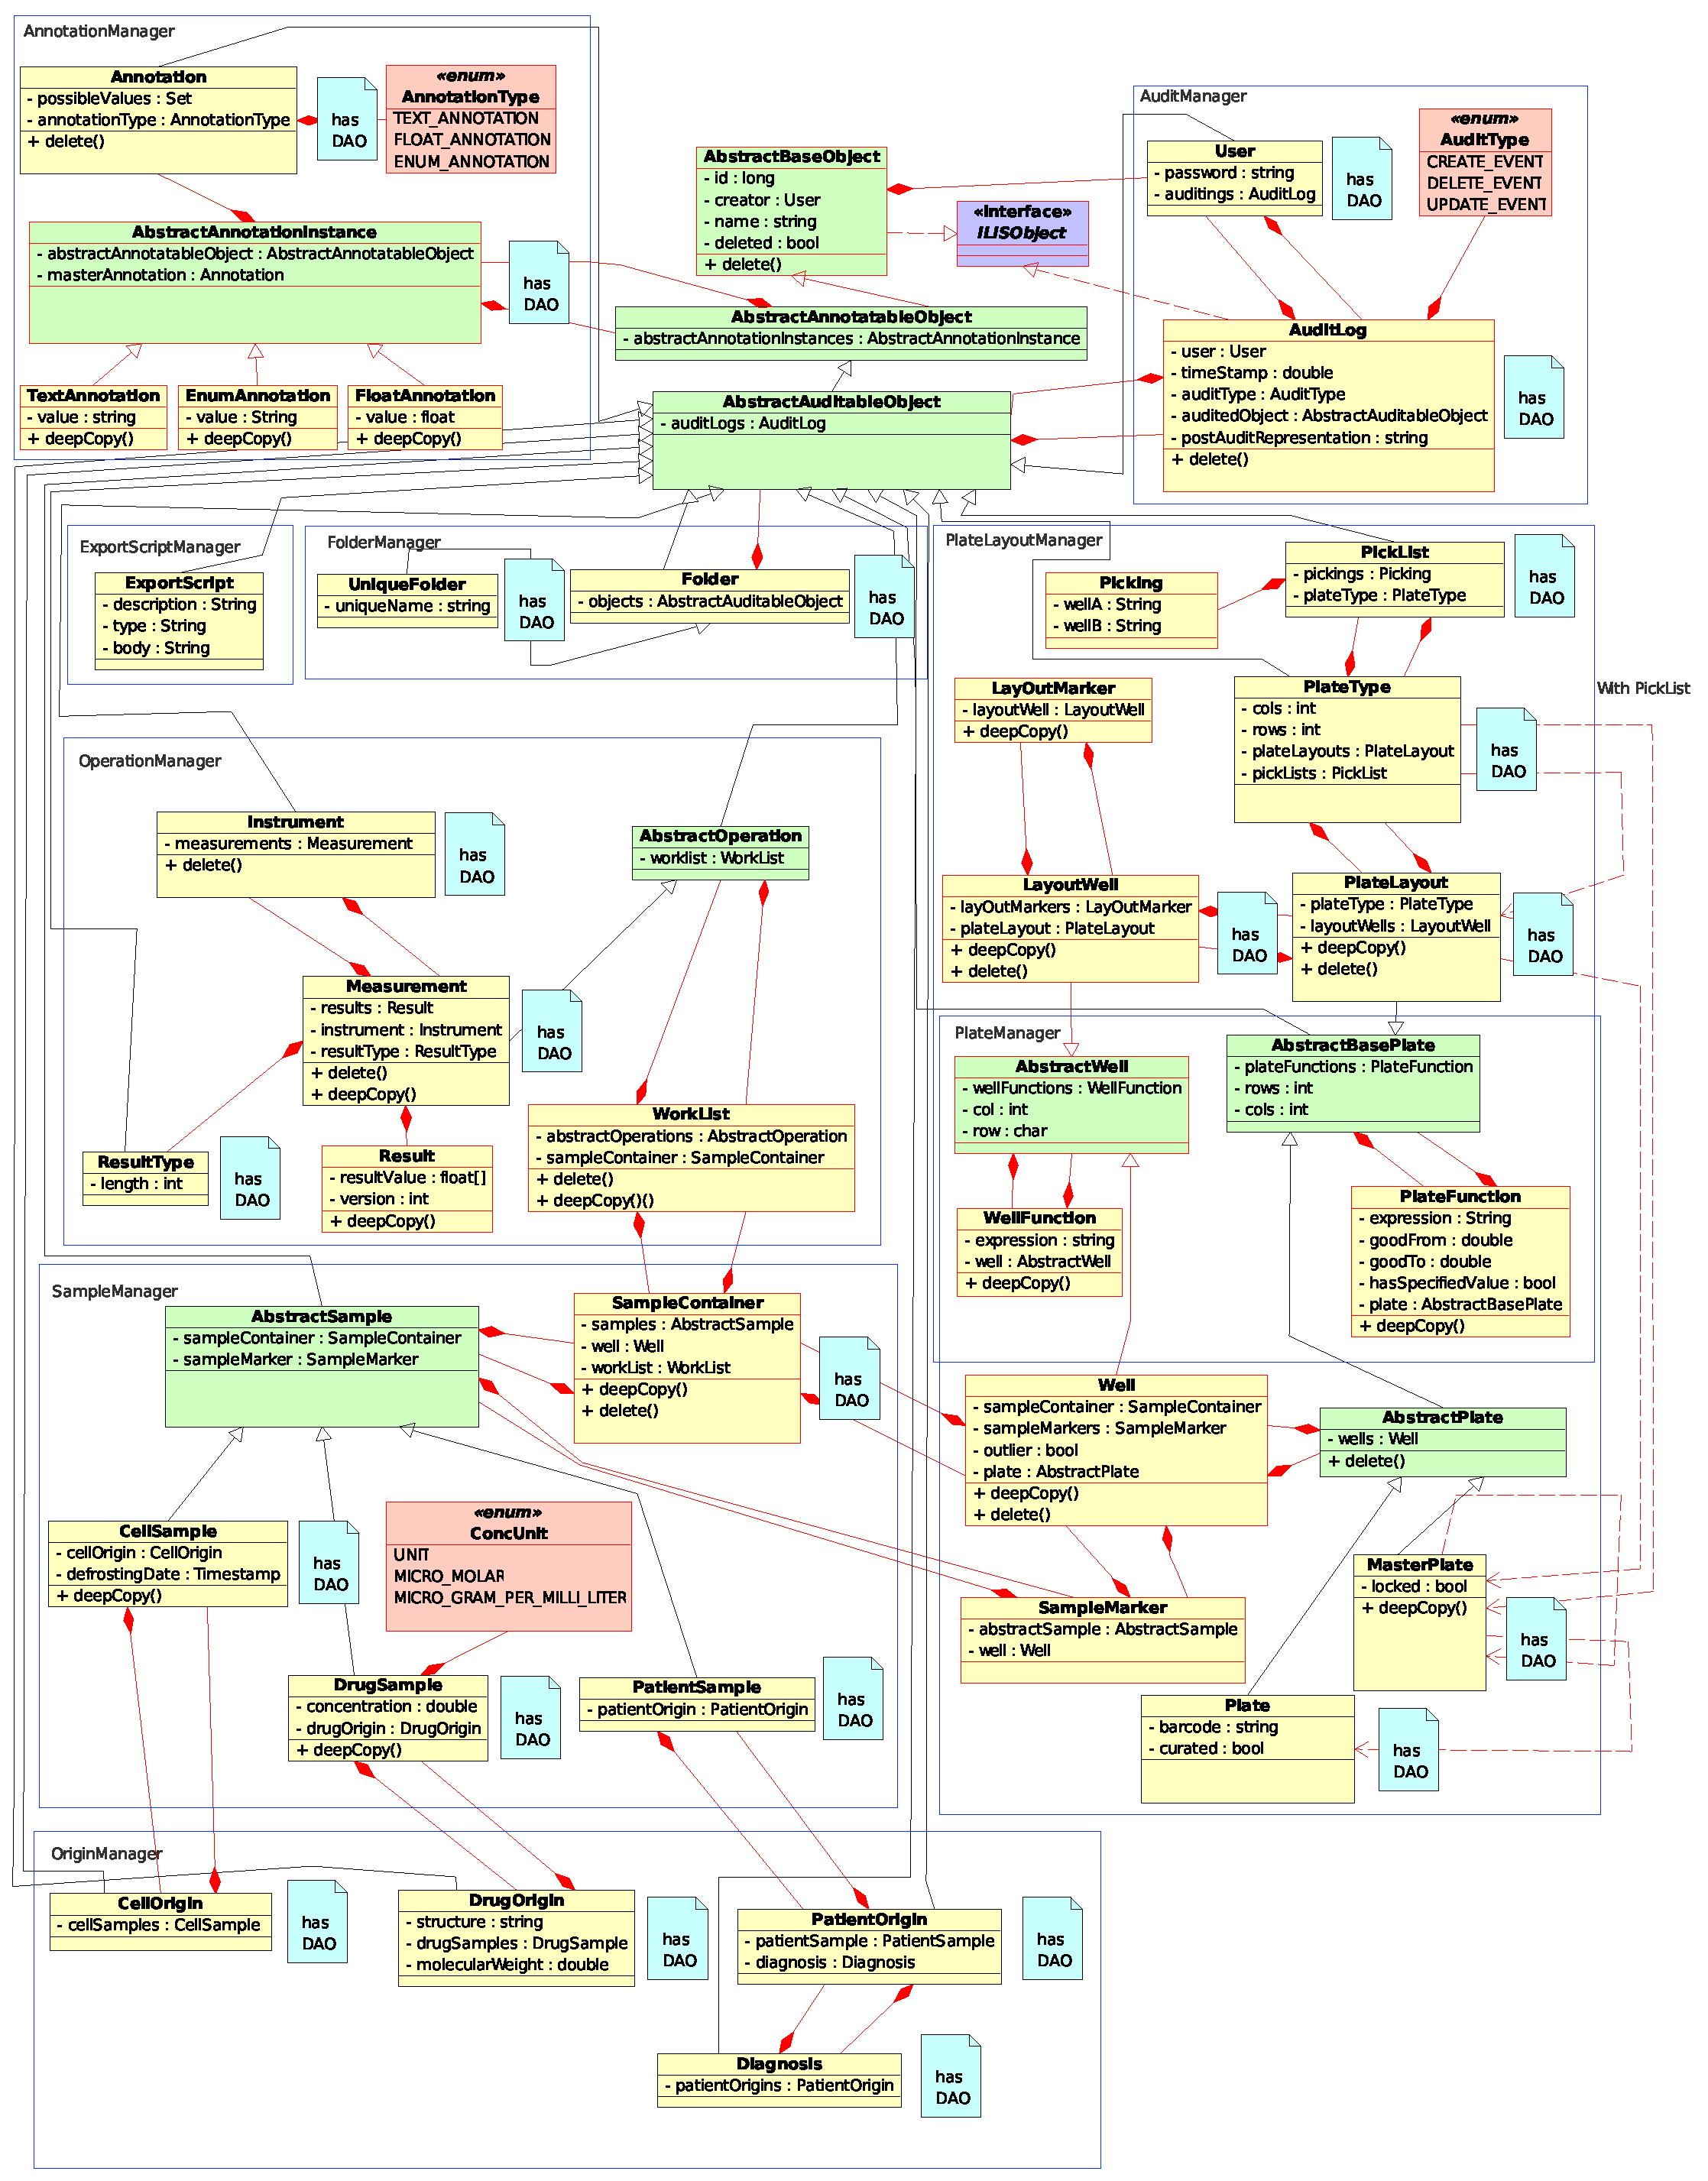
\includegraphics[width=1\textwidth]{UML/classDiagram.eps}
        \end{center}
        \caption{A class diagram of the persistent classes. All classes extend
            \texttt{AbstractBaseObject} (except AuditLog) and some (with black
            frame in figure) also \texttt{AbstractAuditableObject}. The blue
            boxes show which classes are handled by which managers.}
        \label{classdiagram}
    \end{figure}

	\section{Data Access Objects (DAOs)}
	
	\begin{multicols}{2}
        \noindent The data access objects handles the storing and retreaving of
        objects from the database. They are all instances of the class
        \texttt{GenericDAO} (seen in figure \ref{dao}) which use \textsl{Java
        5} generics and \textsl{Spring} AOP introductions to deliver the
        correct object without need for casting and to connect methods declared
        in an interface to \textsl{Hibernate} queries. It also uses the
        \textsl{Spring} class \texttt{HibernateDaoSupport}\footnote{
        \texttt{org.springframework.orm.hibernate3.support.HibernateDaoSupport}}
        as a base because it more or less already contains all the
        functionality.
	    
        Creating a new DAO consists of the following steps:
	    
        \begin{itemize} 
            \item Write an interface for the class where methods
                  that should refer to a \textsl{Hibernate} query begins with
                  the word ``find".  
            \item Write a \textsl{Spring} bean for the class in 
                  \textit{applicationContext.xml}.  
            \item Write the \textsl{Hibernate} query in namedQueries.hbm.xml
        \end{itemize}
    \end{multicols}

    \begin{figure}[p]
        \small{	
        \begin{Verbatim}[frame=single, framerule=0.1pt, framesep=4mm]
package net.bioclipse.lis.genericDAO;

import java.lang.reflect.Method;
import java.util.List;
import net.bioclipse.lis.pojos.IAbstractBaseObject;
import org.hibernate.Query;
import org.springframework.orm.hibernate3.support.HibernateDaoSupport;

/**
 * This class is the basis for the daos. It uses generics to be able to return
 * daos without need for casting. Spring uses it as base to build from when 
 * implementing the dao interfaces. It also contains some methods for running 
 * the correspondingly named Hibernate query when methods defined in the DAO 
 * interface are called.
 * 
 * @author jonathan
 *
 * @param <T> The type of the persistent class the dao object should work with.
 */
public class GenericDAO<T> extends HibernateDaoSupport 
                           implements IGenericDAO<T>, FinderExecutor {

	private Class<T> type;
	
	public GenericDAO(Class<T> type){
		this.type = type;
	}
	
	public void delete(long id) {
	    IAbstractBaseObject obj = (IAbstractBaseObject)getSession().get(type, id);
	    obj.delete();
	    getSession().save(obj);
	}

	public T getById(long id) {
		return (T)getSession().get(type, id);
	}
 
	public void save(T instance) {
	    getSession().saveOrUpdate(instance);
	}
	
	public List<T> executeFinder(Method method, final Object[] queryArgs) {
	     String queryName         = queryNameFromMethod(method);
	     Query namedQuery         = getSession().getNamedQuery(queryName);
	     
	     for( int i = 0; 
	          i < (queryArgs == null? 0 : queryArgs.length);
	          i++
	        ) {
	             Object arg = queryArgs[i];
	             namedQuery.setParameter(i, arg);
	      }
	      return (List<T>) namedQuery.list();
	}

	public String queryNameFromMethod(Method finderMethod) {
		return type.getSimpleName() + "." + finderMethod.getName();
	}
}
        \end{Verbatim}
        }
        \caption{The \texttt{GenericDAO} class}
        \label{dao}
    \end{figure}

	\newpage
	
	\section{Managers}
	\begin{multicols}{2}
    	\noindent
    	The manager classes contains the methods that the GUI will run. They
    	contain the needed DAOs and will forward requests to the right class
    	so that they will be performed. 
    \end{multicols}

%	\begin{figure}[htp]
%	    \begin{center}
%	    	\includegraphics[width=1\textwidth]{UML/Managers.eps} 
%	    \end{center}
%		\caption{A class diagram showing the different manager classes}
%		\label{managares}
%    \end{figure}

	\section{Auditing}
	\begin{multicols}{2}
    	\noindent
    	When an auditable object is created, edited or marked as deleted an
    	auditlog is created. When a non-auditable object that is a part of an
    	auditable object is created, for example a PlateFunction, this happening
    	will be audited as an editing of the auditable object in this case a
    	Plate, MasterPlate or PlateLayout. Table \ref{auditservicecallers}
        contains a list of all the methods that needs to call the AuditService.
        The test AuditInvokedTest checks that all of these calls takes place and
        the test TransactionTest checks that they are in a transaction meaning 
        that either	both the auditing and the actual operation takes place or 
        else neither.
    \end{multicols}

	\begin{table}[hbt]
	
	\begin{center}
    \footnotesize{
	\begin{tabular}{|l|l|}
       	
    		\hline
    		\textbf{Manager} & \textbf{Method} \\
    		\hline
    		\hline
				AnnotationManager & newAnnotation \\
				                  & annotate \\
				                  & delete AbstractAnnotationInstance \\
				                  & delete Annotation \\
				                  & edit AbstractAnnotationInstance \\
				                  & edit Annotation \\
    		\hline
				AuditManager & newUser \\
				             & edit User \\
				             & delete User \\
    		\hline
				OperationManager & newInstrument \\
				                 & newResultType \\
				                 & newMeasurement \\
				                 & edit Measurement \\
				                 & edit Instrument \\
				                 & edit ResultType \\
				                 & delete Measurement \\
				                 & delete Instrument \\
				                 & delete ResultType \\
 				                 & addResult \\
    		\hline
    			OriginManager & createDrugOrigin \\
    			              & createCellOrigin \\
    			              & edit DrugOrigin \\
    			              & edit CellOrigin \\
    			              & delete DrugOrigin \\
    			              & delete CellOrigin \\
    		\hline
    			PlateManager & createPlate \\
    			             & createMasterPlate \\
    			             & createWellFunction \\
    			             & createPlateFunction (with good between values) \\
    			             & createPlateFunction (without good between 
                               values) \\
    		\hline
    			PlateLayoutManager & createPlateType \\
    			                   & createPlateLayout \\
    			                   & createWellFunction \\
    			                   & createPlateFunction (with good between
                                     values) \\
    			                   & createPlateFunction (without good between
                                     values) \\
    		\hline
    			ProjectManager & createProject \\
    			               & createExperiment \\
    		\hline
    			SampleManager & addNewCellSampleToContainer \\
    			              & addNewDrugSampleToContainer \\
    		\hline
	    \end{tabular}
	}
		\end{center}
		
	   	\caption{All methods needing to call the AuditService.audit method. }
	   	\label{auditservicecallers}
	\end{table}
	
    \section{GUI}
        \subsection{Viewing a plate}

            In a couple of different places in the GUI something that shows
            data related to a plate is needed. Table \ref{plateView} lists them
            and what are needed of them.

            \begin{table}[hbt]
            
            \begin{center}
            \begin{tabular}{|l|l|l|}
                
                \hline
                \textbf{Needed to show} &
                \textbf{Seems to be working on} &
                \textbf{Can work on} \\
                \hline
                \hline
                Markers &
                PlateLayout &
                PlateLayout \\

                \hline

                Which calculation functions are defined for a certain well &
                PlateLayout &
                PlateLayout \\

                \hline
                
                Markers and concentrations &
                MasterPlate &
                AbstractPlate \\

                Markers and concentrations &
                Plate &
                AbstractPlate \\

                \hline
                
                Results as numbers &
                Plate &
                Plate \\

                Results as colours &
                Plate &
                Plate \\
                
                \hline
            \end{tabular}
            \end{center}
            \caption{The different situations calling for some kind of
                     plateviewer in the gui.}
            \label{plateView}
            \end{table}
    
	\section{Problems and solutions} 
    \begin{multicols}{2}
        \subsection{Regarding contains-method on HashSet's} During testing the
            following strange thing happened. A set containing an object
            returned false when contains was called with a reference to the
            actual same object. After some consideration the following cause
            was realised. The object was created with a hashcode method using
            some properties of the object. Then those properties of the object
            where changed and finally the contains method was called with the
            changed object thus causing the contains method to perform a lookup
            in the hash ``bucket'' corresponding to the new hashcode and of
            course not finding the object.  The exact effects of this
            phenomenon are not yet realised but it is a good thing to know. The
            current solutions in the test case consists of either making all
            changes before the object is put in the hashSet or saving the
            object to the database followed by reloading the object containing
            the Set from the database and thus getting a new corrrect one.
            This phenomenon is important to have in mind when using HashSet's.

        \subsection{Regarding simultaneous object editing}
            If the original object differs from in the database when the edited
            object is saved a dialog should inform the user who has edited and
            what has changed and allow him to force overwrite or reload and
            redo the changes manually.
    \end{multicols}        
\end{document}
	
